\section{Experiments and Results}

Figure \ref{fig:gilbert2d_examples} and Figure \ref{fig:examples3d} show examples of Gilbert curves for 2D and 3D respectively.

We would like to highlight the ability of the the Gilbert curve to preserve locality analagous to the the Hilbert curve.
To do this, we create plots of average distance in embedded 2D and 3D dimension relative to the linear distance along the curve.
To allow for plot comparison, linear curve distances are normalized, the cumulative sum of average embedded distance is
used which is then modulated by the scaling function $x^{-1-\frac{1}{d}}$.

Algorithm \ref{alg:bin_and_datacollapse} gives pseudo code detailing this process.

\begin{algorithm}
  \caption{ \hskip0.5em Cumulative Binning and Data Collapse }
  \label{alg:bin_and_datacollapse}
  \begin{algorithmic}
    \State Create curve in dimension $D$, $N = |\alpha| \cdot |\beta| \cdot |\gamma|$
    \State Initialize $B = \{0\}^N$, $S = \{0\}^N$, $M=0$
    \State \textit{\# $p_i, p_j$ points in embedded dimension (2D or 3D)}
    \ForAll{ $i, j \in \{0, \dots, N\} \ \ \to p_i,p_j \in \mathbb{Z}^D$}
      \State $B_{ |i-j| } \leftarrow B_{|i-j|} + |p_i - p_j|$
      \State $M \leftarrow M + 1$
    \EndFor

    \ForAll{ $k \in \{1, \dots, N\}$ }
      \State $ x \leftarrow \frac{k}{N} $
      \State $S _ {k} \leftarrow \frac{S _ {k-1} + B _ {k}}{M}$
      \State $G ( x ) \leftarrow \frac{ S _ {k} }{ x^{1 + 1/D} }$
    \EndFor


  \end{algorithmic}
\end{algorithm}

\begin{figure}[h]
  \centering
  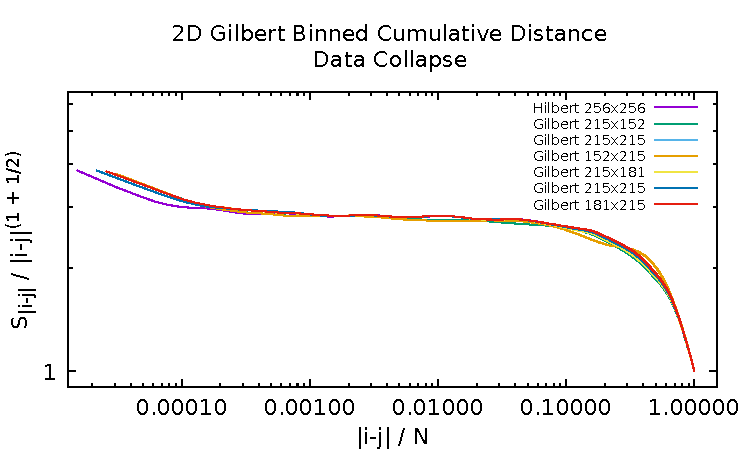
\includegraphics[width=\linewidth]{datacollapse_2d.pdf}
  \caption{ The data collapse for the 2D Hilbert curve of 256x256 and the Gilbert curve of combinations for $((215,152,181) \times (215,152,181))$. 
  Note that the plot is on a log-log scale.
  The middle flat region indicates the scaling function of $|i-j|^{1 + 1/2}$ is chosen correctly.
  The upward bend as the plots approeach $x=0$ and the dip as the plots approach $x=1$ indicate finite-size scaling effects where the distances
  hit the base recursion level or have lengths that span a significant portion of the whole curve.
  See text for more details.
  }
  \label{fig:datacollapse_2d}
\end{figure}

\begin{figure}[h]
  \centering
  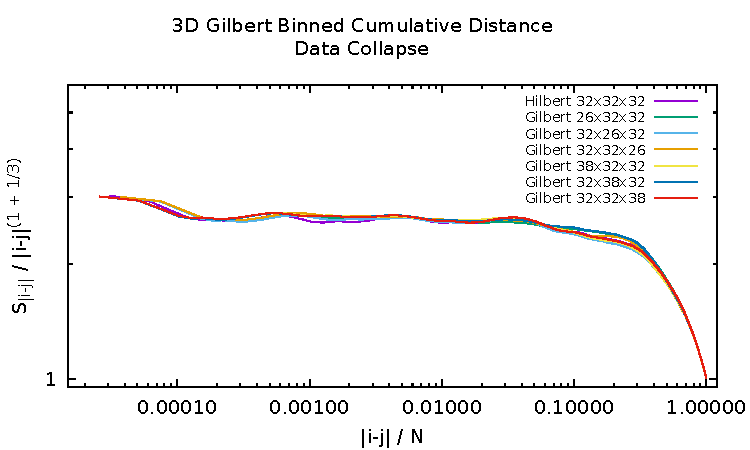
\includegraphics[width=\linewidth]{datacollapse_3d.pdf}
  \caption{ The data collapse for the 3D Hilbert curve of 32x32x32 and the Gilbert curve of combinations for $((26,32,38) \times (26,32,38) \times (26,32,38))$. 
  Note that the plot is on a log-log scale.
  The middle flat region indicates the scaling function of $|i-j|^{1 + 1/3}$ is chosen correctly.
  The upward bend as the plots approeach $x=0$ and the dip as the plots approach $x=1$ indicate finite-size scaling effects where the distances
  hit the base recursion level or have lengths that span a significant portion of the whole curve.
  See text for more details.
  }
  \label{fig:datacollapse_3d}
\end{figure}

\begin{figure}[h]
  \centering
  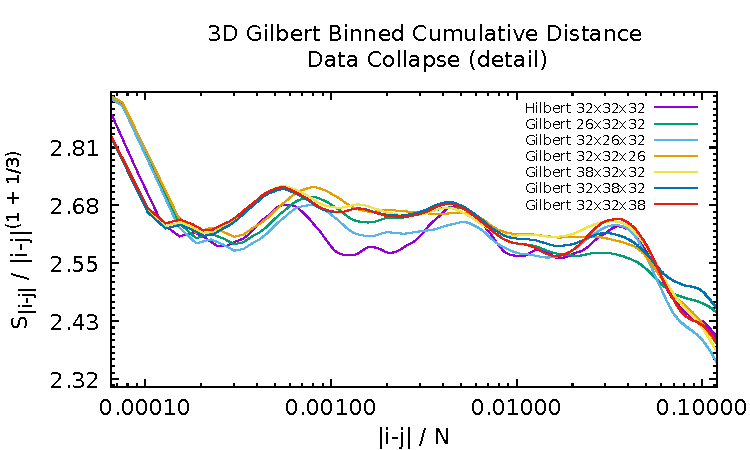
\includegraphics[width=\linewidth]{datacollapse_3d_detail.pdf}
  \caption{ A detail of Figure \ref{fig:datacollapse_3d} restricted to $x = \{6.5 \cdot 10^{-5}, 0.15\}$ and $y = \{2.3,3\}$.
  This higlights ripples in the Hilbert curve as well as fluctutations in the Gilbert curve away from the scaling function.
  These fluctions are minor and could be artifacts of the recursive cuboid subdivision process.
  See text for more details.
  }
  \label{fig:datacollapse_3d_detail}
\end{figure}

Various choices of width, height and depth were chosen for 2D and 3D Gilbert curves and
Algorithm \ref{alg:bin_and_datacollapse} was run on each.
Figures \ref{fig:datacollapse_2d} and \ref{fig:datacollapse_3d} show the overlaid plots
after the data collapse process, showing good agreement to the Hilbert curve.

From the figures, the Gilbert curve can be seen to have good locality properties in
agreement with the Hilbert curve.

The flat, mostly linear region in the middle, from $x \in (0, 0.1]$, indicates a proper scaling
function chosen.
The intuition behind the linear, flat region is that for an index distance along the curve,
this should map to an area or volume in the embedded 2D or 3D space, respectively.
This means that for index position $i$ and $j$ with respective embedded mapped points $p_i$ and $p_j$:

$$
\begin{array}{ll}
  & |i-j| \propto |p_i - p_j|^d \\
  \to & |i-j|^{\frac{1}{d}} \propto |p_i - p_j| \\
\end{array}
$$

Where $|p_i - p_j|$ is the standard Euclidean norm.

Since we take the cumulative distance, this adds one in the exponent for a scaling factor of $x^{-1-1/d}$,
for dimension $d = (2,3)$.
Fluctuations away from the scaling factor indicate a failure for the curve to be space filling.
Significant fluctiations can be seen near the ends of the plots when the binning technique
succums to finite-size scaling effects.
For Figures \ref{fig:datacollapse_2d} and \ref{fig:datacollapse_3d} this happens when the distances
are close to the base recursion level or when the index distances are significantly proportional to
the size of the curve.

Though the Hilbert and Gilbert curve are space filling, there are minor fluctuations from the scaling
function that can be seen in the detail view Figure \ref{fig:datacollapse_3d_detail}.

We note that the data collapse plot for the Hilbert curve has ripples, which
we suspect is an artifact of the square recursive procedure of how
the Hilbet curve is constructed.
Other than to make a note of it, we don't pursue investigation of these ripples in the Hilbert curve
or the minor fluctions from the scaling function in the Gilbert curve further.


